\chapter{Architektúra}

\section{A robot topológiája}

A robot tervezése sok kisebb feladatból és megtervezendő egységből, alegységből
áll. A tervezés során célravezető megközelítésnek tartottam a nagyobb egységek
megtervezésétől a kisebb alegységek megtervezéséíg haladni. Így a specifikációtól
indulva az aktuális feladatot alfeladatokra bontva volt lehetőségem kidolgozni a
robot részleteit annélkül, hogy a részletekben nagyon elvesznék.

Ezt a megközelítést követve a specifikáció alapján meghatároztam a modulokat,
amiket a robot működéséhez létre kell hozni. Ezt követően meghatároztam az
interfészeket, amin a modulok egymással kapcsolatban állnak, maje ezekből egy
diagrammot készítettem, amelyen a rendszer áttekinthető. A
~\ref{fig:robot-diagram-simple} ábra szemlélteti az első elképzelést, ahol a
legnagyobb hardveres modulokat ábrázolom funkciójuk szerint.

\begin{figure}
  \centering
  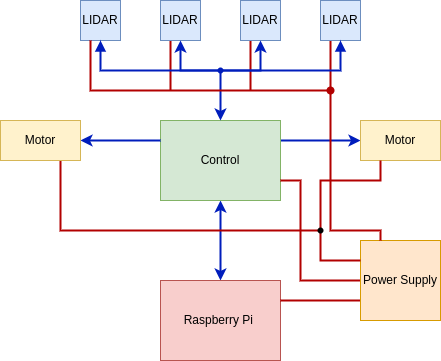
\includegraphics[width=100mm, keepaspectratio]{figures/ch2/robot-diagram-simple.png}
  \caption{A robot egyszerű diagrammja}
  \label{fig:robot-diagram-simple}
\end{figure}

\subsection{A Differenciális robot}

A tervezés első fázisa a robot kialakításának kiválasztása volt. Az autonóm
robotok számos elrendezésben megtervezhetők, amely a robot alkalmazásától függően
lehet komplexebb vagy egyszerűbb. Bizonyos környezetek robosztusabb kialakítást
igényelnek, más környezetek nagyobb mozgékonyságot. A projekt szempontjából a
differenciális elrendezést tartottam a legcélravezetőbbnek.

Az autonóm robotok között a differenciális robot egy relative könnyen
megvalósítható konstrukció, így a projekt fokuszában egy ilyen konstrukció
mellett maradtam. Ennek a robot típusnak összesen két motor áll rendelkezésére
hogy helyzetét és orientációját változtassa, ezáltal könnyebben megvalósítható
mint komplexebb meghajtással rendelkező társai, viszont mozgékony és sok
lehetőséget tartogató kialakítás.

\begin{figure}
  \centering
  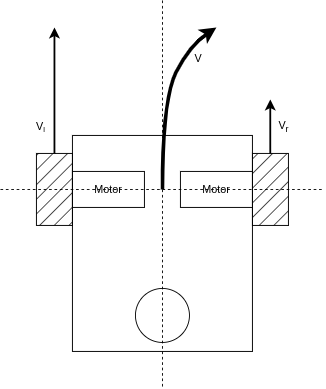
\includegraphics[width=100mm, keepaspectratio]{figures/ch2/diff_robot.png}
  \caption{A differenciális robot kialakítása}
  \label{fig:diff-robot}
\end{figure}

Klasszikus elrendezése, hogy a két motort a hosszanti tengellyel merőlegesen kell
elhelyezni, ezálal a a robot sebessége a motorok szögsebességéből valamint a
kerékátmérőből számítható. A robot orientációját a két motor különböző nagyságban
és/vagy különböző irányban történő meghajtásával lehet vezérelni.

A kialakítás további előnyeihez tartozik, hogy a robot vezérléséből csak relative
kevés erőforrást kell a mozgásra allokálni, hiszen pusztán csak a két motorhoz
tartozó szabályozó és irányító algoritmusokat kell futtatni, ugyanakkor a robot
sík, vagy közel sík terepen minden különösebb nehézség nélkül képes navigálni,
ezáltal sokféle alkalmazásban ideális választás lehet.

\subsection{Modulok és feladatkörök}

A robot megalkotását modulok megtervezésére és realizációjára alapoztam, ennek a
megközelítésnek a tervezésen kívül a végtermék minőségében is jelentős hatásai
voltak. A kész robot ugyanis különálló, de jól meghatározott interfésszel
rendelkező modulok összességéből áll össze, így ha egy alkatrész meghibásodik,
vagy a minősége nem megfelelő, az eszközt könnyebben lehet javítani, vagy a hibás
modult cserélni. Ezen felül, amennyiben új elvárás merülne fel, úgy kevés
alkatrész cseréjével, vagy újak implementálásával könnyen alkalmassá tehető a
robot, egyéb feladatok ellátására is.

A projekt ennek a megközelítésnek köszönhetően könnyen fejleszthető, amennyiben
igény merülne fel adott modulok letisztázására, vagy funkcióköreik bővítésére. A
szóban forgó modul ugyanis, ameddig betartja a számára meghatározott interfészt,
minden különösebb nehézség nélkül fejleszthető és módosítható úgy, hogy a robot
működőképes marad.

\begin{figure}
  \centering
  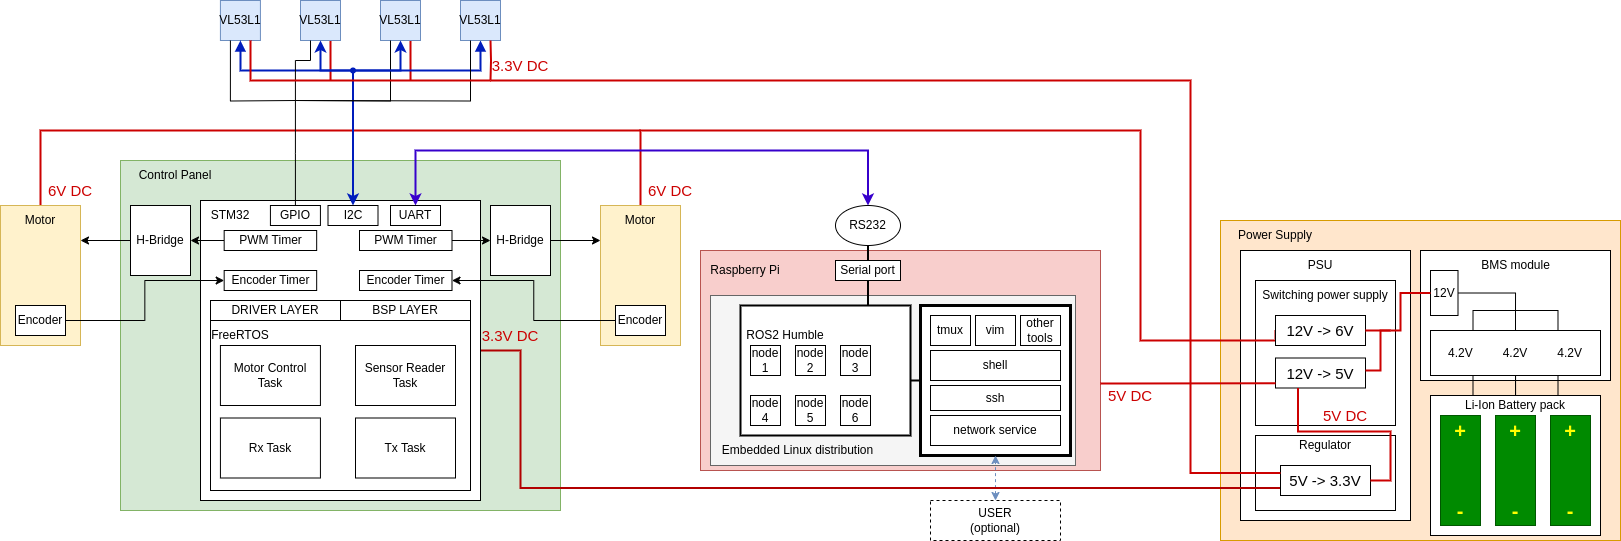
\includegraphics[width=150mm, keepaspectratio]{figures/ch2/robot-diagram-complex.png}
  \caption{A robot komplex diagrammja}
  \label{fig:robot-diagram-complex}
\end{figure}

\medskip

A~\ref{fig:robot-diagram-complex} ábrán látható, a robot moduljainak részletesebb
felosztása amelyen bemutatom a modulokat. Ezen az ábrán már megfigyelhetőek a
szoftveres modulok egyszerűsített ábrái is, így ezeket a fizikai kialakítással
egy ábrán szemlélve jobban átlátható a rendszer.

\subsubsection{A tápellátás kialakítása}
A~\ref{fig:robot-diagram-complex} és~\ref{fig:robot-diagram-simple} ábrákon
narancssárga színnel jelöltem a tápellátásért felelős modult. Ennek a modulnak
több kisebb alegysége van, amelyek a szükséges feszültségszintek előállításának
más-más részeiért felelnek.

\medskip

Az akkumulátorpakk a rendszer energiatároló modulja. A robot három darab 18650-es
méretű akkumulátor befogadására képes, melyeket az ábrán zöld színnel
jelöltem. Az akkumulátorok Lítium ion alapú akkumulátorok, amelyek nagy
népszerűségnek örvendenek. Ezek a cellák teljesen feltöltött állapotban 4.2V
feszültséget biztosítanak, és merülésükkel sem csökken számottevő mértékben a
kapocsfeszültség. A három cella biztosítja a megfelelő bemenő feszültségszintet
és teljesítményt a tápegyég számára, és a robot feladatához mértem megfelelő
kapacitással is rendelkezik. Az akkumulátorok kiválasztásánál fontos szempont
volt, hogy a cellák képesek legyenek a rendszer által igényelt 30W teljesítmény
leadására is.

\medskip

A lítium alapú akkumulátorok hátrányai közé tartozik, hogy alkalmazásukkor
kiegészítő védőáramköröket kell használni, mert illesztésük komplex feladat, és
nem megfelelő használat esetén az akkumulátor hőt fejleszt ami veszélyessé
teheti. Erre a célra a tápellátó modul egy BMS\footnote{BMS:~Battery Management
System} modult is tartalmaz, amely a három cella menedzselését, és illesztését
végzi. A modul a kimenetein 12.6V DC feszültséget biztosít (teljesen feltöltött
cellák esetén), amely már alkalmas bemenet a tápegység számára.

\medskip

A tápegység a bemenetére kapcsolt 12V DC feszültségből a rendszer által igényelt
feszültségszintek előállításáért felelős modul. A kapcsolás az előző fejezetben
ismertetett módon működik: két kapcsolóüzemű tápegységből, egy LDO-ból, valamint
a hozzájuk tartozó kiegészítő elektronikából áll. A kimeneti feszültségei 3.3V,
5V és 6V, amelyeket a robot vezérlése, szenzorai, és motorjai igényelnek.

A tápegység szintén 30W teljesítményre lett méretezve, ez a 6V-os kimeneten 15W
és az 5V-os és 3.3V-os kimeneteken összesen 15W teljesítmény arányában oszlik
meg. 

\subsubsection{A szenzorok és a meghajtás}

A robot két fő komponenstípus segítségével végzi a feladatát. Az egyik a
bevezetőben bemutatott VL53L1 LIDAR szenzor, amely a falaktól és a környezet
egyéb objektumaitól való távolság meghatározására szolgál, a másik a hely- és
pozícióváltoztatásra alkalmas szervó motor. A bevezetőben ezek a komponensek már
bemutatásra kerültek, itt az alkatrészek integrációjáról ejtenék pár szót.

\medskip

A motorok meghajtásához a vezérlőpanelen két H-bridge meghajtó áramkört
alkalmaztam. Ezek bemenete a motorok által igényelt feszültség, valamint két
logikai feszültségtartományba eső PWM jel, amelyek a hídkapcsolás irányát
befolyásolják, valamint kitöltési tényezőjükkel a motort meghajtó
teljesítményértéket állítják be. A motorok tápfeszültségét, a vezérlő panel
továbbítja a tápegység felől, a PWM jelek előállításáért pedig a vezérlőpanelen
található mikrokontroller felel.

A motorok rendelkeznek beépített enkóderrel, amelyeket szintén a vezérlőpanelen
található mikrovezérlő kezel.

\medskip

A~\ref{fig:robot-diagram-simple} ábrán látható, hogy a robot négy szenzort
használ fel a tájékozódásra. A LIDAR szenzorok I2C buszon kapcsolódnak a
mikrovezérlőhöz, amin keresztül vezérlésük végezhető, valamint a mért értékek
kiolvasható. A SATEL boardok számára a szükséges 3.3V tápfeszültséget a
vezérlőpanel továbbítja.

A választott mikrokontroller nem tartalmaz annyi I2C perifériát, mint ahány
szenzor illesztését a feladat megkövetelné, így alternatív megoldást kerestem. A
szenzorok rendelkeznek módosítható cím funkcióval, így ezt a megoldást ítéltem a
legkézenfekvőbbnek. A modulok rendelkeznek egy XSHUT nevű kivezetett lábbal,
amely funkciója az adatlap alapján, hogy az eszköz bootolását befolyásolja. Ennek
a lábnak a felhasználásával az egyes szenzorok az inicializációs fázisban
egyesével bootolhatóak, ami lehetővé teszi a firmware számára, hogy egyedi I2C
címeket rendeljen minden eszközhöz. Ennek érdekében négy GPIO lábat felhasználtam
a szenzorok vezérlésére.

\subsubsection{A vezérlőpanel}

A panel egyetlen tápcsatlakozó bemenettel rendelkezik, amelyen a szükséges 3.3V
és 6V feszültségeket a tápegységtől megkapja. Ezeket a feszültségeket innen
továbbítja a megfelelő komponenseknek. A csatlakozás a robot többi komponenséhez
a panel szélén található tüskesor csatlakozókkal történik.

\medskip

A vezérlő panel hordoz két H-bridge meghajtó áramkört, amelyeket a motorok
vezérlésénél már említettem. Ezek az áramkörök a panelen található mikrovezérlő
lábaira csatlakoznak, amiken a vezérlőbe épített timer periféria PWM jellel képes
őket vezérelni. Az integrált áramkörök kimenete a panel jobb és bal oldalán
található csatlakozókhoz kapcsolódik, ahol a vezérlőpanelt vezeték köti össze a
motorokkal.

\medskip

A vezérlőpanel hordozza a motorok vezérlését, és szenzorok olvasását végző
mikrovezérlőt. A kontroller több szempontból is előnyös választásnak bizonyult. A
mikrovezérlő teljesítmény szempontból alkalmas a feladat ellátására valamint
perifériák számában és minőségében is elegendő erőforrással rendelkezik. A
kontrollercsaládról ezen felül rendelkezem és előzetes tapasztalattal is.

A mikrokontroller típusát tekintve egy STM32F103C8 mikrovezérlőre
esett a választás, amely egy Cortex-M3 maggal rendelkező
mikrovezérlő. Ez a modell rendelkezik több USART és I2C perifériával,
valamint TIMER perifériái támogatják az enkóder módot és PWM
generálást, amely a motorok vezérlésére, valamint az enkóder jelek
feldolgozására alkalmas. Az I2C periféria alkalmas a szenzorok
illesztésére, az USART periféria pedig debug célokra a fejlesztési
fázisban, illetve a Raspberry Pi-vel történő kapcsolattartásra
alkalmas\cite{stm32source}.

A mikrovezérlő mellé a gyártó CMSIS támogatást biztosít (ARM magú chipről lévén
szó) valamint külön hardver absztrakciós könyvtárat, amely a konfigurálást és a
hardverek kezelését könnyebbé teszi. Az ábrán egy egyszerűsített és limitált
szemléltetése figyelhető meg a firmwarenek. A kód alapja egy FreeRTOS 32 bites
beágyazott real-time operációs rendszer, amely a multitasking feladatokat nagyban
megkönnyítette. A firmware további tulajdonságait, fejlesztésének menetét a
következő fejezetben bővebben kifejtem.

A vezérlőpanel a központi vezérlő SBC panelhez soros porton keresztül
csatlakozik, ahol saját protokollon keresztül üzenetek váltására van lehetőség. 

\subsubsection{A Rasppberry Pi}

Az ábra utolsó pirossal jelölt blokkja egy Raspberry Pi 4B modell. Az SBC soros
porton keresztül kapcsolódik a vezérlő panelhez, tápellátásáról pedig a tápegység
modul 5V DC csatornája gondolskodik.

A panel egy tüskesorral van szerelve, amelyen keresztül lehetőség van a board
megtáplálására, valamint a soros port is ki van vezetve rá. A többi felszerelt
csatlakozó a projekt során nem volt használva.

\medskip

A kapcsolatot a felhasználó, hálózaton keresztül teremthet a Raspberry Pi-vel,
amire a beépített WiFi modulon keresztül van lehetőség. A WiFi modul képes
accesspoint működésre, ami a robot függetlenségében nagy segítség. A Linuxal
foglalkozó fejezetben a kapcsolódás módjait, valamint a telepített eszközöket
bővebben ki fogom fejteni.

\medskip

A modul fő feladata a humán interfész biztosításán felül egy ROS környezet
futtatása, amin belül a robot funkcionalitása. A soros port a Linux rendszeren
belül egy device file-ként elérhető, amit a ROS környezetből egyszerű
fileműveletekkel használhatunk. Ezen a módon a robot hardvere és vezérlése
közötti kapcsolat megteremthető.\cite{rpisource}

\section{A mechanikus váz}

A robot moduljainak áttekintése után tiszta kép alakult ki arról, hogy a kész
robotnak milyen komponenseket kell tartalmaznia. A fizikai komponensek
összetartására a robot váza, és a rögzítőelemek szolgálnak. 

\subsection{Tervezés}

A váz tervezési fázisát az alkatrészeim geometriai paramétereinek felmérésével
kezdtem. Ezek után több topológiát vázoltam fel, és értékeltem őket
megvalósíthatóság, átláthatóság és anyag-igény szempontjából. A végleges
kialakítás végül egy ``emeletes'' konstrukció lett, amely két alap panelt
tartalmaz, amiket távtartók tartanak egymástól 6 cm távolságban. Ezekre a
panelekre funkcionalitás alapján elrendeztem a robot komponenseit oly módon, hogy
a végleges kialakításban az egyes komponensek hozzáférhetőek maradjanak, de a
robot kompakt kialakítású legyen.

Az alsó panelre kerültek a motorok, és az akkumulátorpakk, ezutóbbi súlyával
biztosította a stabilitást. Az akkumulátorpakk mellett kapott helyet a BMS modul,
valamint a tápegység. A megfelelő teljesítmény biztonságos kihasználása érdekében
AWG24 besorolású vezetékekből készítettem el az összeköttetéseket.

A felső panelre a Raspberry Pi, és a vezérlőpanel kerültek.

A panelek számára legalkalmasabb alapanyagnak a rétegelt fa lemezt tartottam,
amelyet könnyen megmunkálhattam. Az összeszerelésre metrikus csavarokat és
kompatibilis fém távtartókat választottam, amelyek méretüket tekintve az
áramkörök furatainak megfeleltek.

A tervezésben a kezdeti koncepció kialakítása után proof of concept jellegű 
3D modelleket készítettem a FreeCAD tervezőszoftver segítségével, amelyek
segítségével a robot összeszerelése előtt ellenőriztem a méretkorlátokat és a
helyigényt.

\subsection{Megvalósítás}

A pontos tervek kialakítását követően megrendeltem az alkatrészeket, és
összeszereltem a robotot.

\section{A terv értékelése}

A robot kialakítása és megtervezése során felmerültek olyan fejlesztési és
javítási kérdések, amelyek már nem voltak időben megvalósíthatóak, ezeket mutatom
most be.

A firmware, yocto és Linux, valamint a ROS2 modulokhoz tartozó fejlesztési
lehetőségeket, hibákat és értékelést az adott témához tartozó fejezetben
részletezem.

\subsection{Pozitívumok}

A projekt moduláris megközelítéséből nagyon sokat profitáltam, a feladatok
ugyanis bizonyos megkötésekkel párhuzamosíthatóak voltak, ami a fejlesztést
nagyban gyorsította és tette kényelmesebbé. Egy késleltetett rendelés például nem
akasztotta meg teljesen a munkát, csak egy részmodult késleltetett.

\medskip

Az adott modulok tesztelése szintén sokkal könnyebbnek bizonyult úgy, hogy egy
előre defíniált interfészt vagy protokollt tudtam követni. Így egy feladatot
könnyebben lehetett elvégezettnek tekinteni ha a tesztelésen átesett, nem kellett
az egész konstrukciónak elkészülnie a részeredményekhez. 

\subsection{Hátrányok}

Az előre defíniált interfészek jelentettek nehézséget is. Ha egy modul
fejlesztésében nem várt nehézséget okoz egy bizonyos interfész betartása, akkor
az sok fejlesztési idő kiesését tudja jelenteni.

A projekt fejlesztése nagyon erősen függ olyan döntésektől amikben a fejlesztést
megelőzően kevés tapasztalattal rendelkeztem, hogy hatékony interfészt határozzak
meg. Ilyen esetben vagy a már meglévő modulokhoz alkalmazkodva több idő és
energia ráfordítással fejlesztettem le a modult, vagy módosítottam az interfészt,
amennyiben nem, vagy csak nagyon kevés modul függött az adott interfésztől. Az
utólagos interfészmódosítások azonban nagy bizonytalansággal járhatnak, és a
legtöbb esetben érdemes azokat elkerülni.

\medskip

A fizikai kialakítás során sok munkát jelentett a kábelezés megvalósítása.
Gyakran adódott olyan teszt ami azért nem volt sikeres, mert egy kábel
kontaktushibás volt és ezen darabok megkeresése sok időt vett igénybe.

\subsection{Fejlesztési lehetőségek}

A robot mechanikus és hardveres kialakítása sok fejlesztési lehetőséget
tartalmaz. Mind elektronikai, mind mechanikus oldalról léteznek fejlesztési
lehetőségek.

\subsubsection{Elektronika}

A vezérlőpanel, és a tápegység is nélkülözi a táp indikátor LED-et, amely világít
ha az eszköz feszültség alatt van. Ez, bár egy egyszerű kiegészítés, sokszor
megkönnyíti a tesztelést.

\subsubsection{Kábelezés és összeköttetések}

A kábelezés és csatlakozók tekintetében is van tér a fejlődésre. Bár a tüskesor
alapú csatlakozók prototípus esetén kiválóan működnek, és alkalmazásukkal könnyen
javíthatók esetleges félrekötések, a tényleges összerakást gyakran nehezítik
komplexitásukkal. Minden alkatrésznek meghatározott csatlakozó tervezésével, amit
esetleges foglalat felhasználásával egyetlen módon lehet a panelhez
csatlakoztatni, nagy könnyebbséget és átláthatóságot biztosíthatunk az eszköznek.

\medskip

A kétpaneles emeletes elrendezés szintén a kábelezés miatt eredményezett kevésbé
átlátható kialakítást. A panelek közötti kapcsolatra szallagkábel
felhasználásával egy tisztább és átláthatóbb struktúrát eredményez.

\medskip

A panelok összekapcsolása megoldható lenne egy hordozó PCB
segítségével, amely így a közeli panelok közötti összeköttetéseket ugyanúgy
biztosíthatja, ellenben sokkal átláthatóbb marad, ezáltal előnyösebb mint a
jelenlegi megoldás.

\subsubsection{Komplexitás}

Adott modulokkal kapcsolatban, bár feladatukat helyesen látják el, jogosan
merülne fel új funkcionalitásra igény.

\medskip

A tápegység egy tisztán analóg kialakítás, amelynek semmilyen monitorozórendszer
nem része. Egy komplexebb táp kialakításával a robot saját akkumulátorának
állapotáról értesülhetne, esetleges tápkimaradások esetére tartalék
kondenzátorról biztosított leállást is el lehetne érni. 

\medskip

A vezérlőpanel tartalmaz olyan funkciókat amelyek korábbi alkalmazásokhoz
készültek így nincsenek kihasználva. Ennek a függvényében a panel geometriailag
indokolatlanul nagy, a funkciói és komplexitása figyelembevételével.

Az alkalmazott mikrokontroller, bár feladatát ellátja, nélkülözi az FPU
támogatást, amely nagyban nehezíthet, ha a motor komplexebb szabályozására igény
merülne fel.

Az mikrovezérlő órajelforrásként a belső órajelgenerátort használja, egy külső
órajelforrásról ugyanezzel a vezérlővel, 8MHz órajel helyett akár 72MHz órajel is
elérhető, ami sokkal nagyobb tartalékot jelent bármilyen időzítési feladatnál.

\subsubsection{Mechanika}

Az elektronika rögzítésénél nehézséget jelentett a többfajta furatméret. Egy
egységesített furatokkal tervezett konstrukció nagyban megkönnyítené az
összeszerelést.

\bigskip

A fejezetben szó volt a robot kialakításáról és architektúrájáról. Részletesen
bemutattam a robot moduljait, és azok feladatát, valamint egymáshoz való
kapcsolódását. Kitértem a fizikai realizáció lépéseire, kihívásaira. Végül a kész
produktumot elemeztem hibák, és fejlesztési lehetőségek szempontjából.

A következő fejezetben ismertetem a mikrokontroller firmware-ét, annak
képességeit, és fejlesztésének módját. 

